\documentclass[11pt,letterpaper]{article}

% Fonts - IBM Plex, the font of Cyberspace
\usepackage[utf8]{inputenc}
\usepackage[T1]{fontenc}
\usepackage{plex-sans}
\usepackage{plex-mono}
\renewcommand{\familydefault}{\sfdefault}

% Layout
\usepackage[margin=1in]{geometry}
\usepackage{multicol}
\usepackage{enumitem}
\usepackage{titlesec}

% Math symbols (for \checkmark)
\usepackage{amssymb}

% Colors - Soft, sophisticated palette
\usepackage{xcolor}
\definecolor{cyberbg}{RGB}{252,251,247}      % Soft white/cream
\definecolor{cyberblue}{RGB}{0,102,204}      % Deep blue
\definecolor{cybergreen}{RGB}{0,128,96}      % Forest green
\definecolor{cybergray}{RGB}{96,96,96}       % Subtle gray
\definecolor{cyberaccent}{RGB}{204,102,0}    % Warm orange
\definecolor{cyberpurple}{RGB}{102,51,153}   % Royal purple

\pagecolor{cyberbg}

% Graphics
\usepackage{tikz}
\usetikzlibrary{trees,positioning,arrows.meta,shapes,shadows,decorations.pathreplacing}

% Hyperlinks
\usepackage{hyperref}
\hypersetup{
    colorlinks=true,
    linkcolor=cyberblue,
    urlcolor=cyberblue,
    pdftitle={Cyberspace Library Structure},
    pdfauthor={Claude Code Librarian}
}

% Custom section formatting
\titleformat{\section}
  {\Large\bfseries\color{cyberblue}}
  {\thesection}{1em}{}

\titleformat{\subsection}
  {\large\bfseries\color{cybergreen}}
  {\thesubsection}{1em}{}

% Custom commands
\newcommand{\directory}[1]{\textcolor{cyberpurple}{\texttt{#1/}}}
\newcommand{\file}[1]{\textcolor{cybergray}{\texttt{#1}}}
\newcommand{\pdfcount}[1]{\textcolor{cyberaccent}{\textbf{#1 PDFs}}}

% Title styling
\usepackage{titling}
\pretitle{\begin{center}\Huge\bfseries\color{cyberblue}}
\posttitle{\par\end{center}\vskip 0.5em}
\preauthor{\begin{center}\large\color{cybergray}}
\postauthor{\end{center}}
\predate{\begin{center}\large\color{cybergray}}
\postdate{\end{center}}

\title{Cyberspace Library}
\author{LaTeX-Style Directory Tree\\{\small The font of Cyberspace: IBM Plex}}
\date{\today}

\begin{document}

\maketitle

\begin{center}

\begin{tikzpicture}
\node[draw=cyberblue,thick,rounded corners,fill=cyberbg,text width=0.9\textwidth,align=center,
      drop shadow={opacity=0.2}] {
  \textbf{\large\color{cyberblue}312 research papers} indexed with \\
  \textbf{\color{cybergreen}LaTeX makeindex-style KWIC permutation} \\
  {\small\color{cybergray}Deduplicated, cross-referenced, hierarchical}
};
\end{tikzpicture}
\end{center}

\vspace{1em}

\section*{Library Structure}

\subsection*{Index \& Metadata}

\begin{description}[leftmargin=2em,style=nextline]
  \item[\file{index.html}] \pdfcount{7,474 lines} — Permuted KWIC Index
  \begin{itemize}[leftmargin=1.5em]
    \item[\color{cybergreen}$\triangleright$] 312 PDFs indexed with clickable links
    \item[\color{cybergreen}$\triangleright$] Deduplicated, alphabetically sorted A--Z
    \item[\color{cybergreen}$\triangleright$] LaTeX makeindex style formatting
  \end{itemize}
\end{description}

\subsection*{Collections}

\subsubsection*{Root Collection --- \pdfcount{186}}

The primary collection spans multiple research domains:

\begin{multicols}{2}
\textbf{\color{cyberblue}Computer Architecture \& Systems}
\begin{itemize}[leftmargin=1em,itemsep=0pt]
  \item[\tiny$\bullet$] Apollo Guidance Computer - BLOCK I
  \item[\tiny$\bullet$] ARM system-on-chip architecture
  \item[\tiny$\bullet$] Intel 64 and IA-32 Architectures
  \item[\tiny$\bullet$] Hardware Memory
\end{itemize}

\textbf{\color{cyberblue}Programming Languages}
\begin{itemize}[leftmargin=1em,itemsep=0pt]
  \item[\tiny$\bullet$] LISP I Programmers Manual (1960)
  \item[\tiny$\bullet$] Bluebook Smalltalk80
  \item[\tiny$\bullet$] The Next 700 Programming Languages
  \item[\tiny$\bullet$] Understanding and writing compilers
\end{itemize}

\textbf{\color{cyberblue}Distributed Systems}
\begin{itemize}[leftmargin=1em,itemsep=0pt]
  \item[\tiny$\bullet$] MapReduce on Large Clusters
  \item[\tiny$\bullet$] In Search of Understandable Consensus
  \item[\tiny$\bullet$] HyperDex Key-Value Store
  \item[\tiny$\bullet$] Deconstructing the Database
\end{itemize}

\textbf{\color{cyberblue}Software Engineering}
\begin{itemize}[leftmargin=1em,itemsep=0pt]
  \item[\tiny$\bullet$] Clean Code
  \item[\tiny$\bullet$] Refactoring (Fowler)
  \item[\tiny$\bullet$] Designing Interactions
\end{itemize}

\textbf{\color{cyberblue}Algorithms \& Data Structures}
\begin{itemize}[leftmargin=1em,itemsep=0pt]
  \item[\tiny$\bullet$] O(ND) Difference Algorithm
  \item[\tiny$\bullet$] Cache-Oblivious Algorithms
  \item[\tiny$\bullet$] Index Compression
\end{itemize}
\end{multicols}

\subsubsection*{\directory{Type Theory - FP - PLT} --- \pdfcount{47}}

\begin{multicols}{2}
\textbf{\color{cybergreen}Type Theory Foundations}
\begin{itemize}[leftmargin=1em,itemsep=0pt]
  \item[\tiny$\circ$] Cardelli: Types
  \item[\tiny$\circ$] Type Theory and Functional Programming
  \item[\tiny$\circ$] Proofs and Types
  \item[\tiny$\circ$] Martin-Löf Type Theory
  \item[\tiny$\circ$] Theory of Programs
\end{itemize}

\textbf{\color{cybergreen}Type Systems}
\begin{itemize}[leftmargin=1em,itemsep=0pt]
  \item[\tiny$\circ$] Type Inference For Recursive Definitions
  \item[\tiny$\circ$] Practical Type Inference (Success Typings)
  \item[\tiny$\circ$] Strong Types for Relational Data
  \item[\tiny$\circ$] Generalized Constraints (C\# Generics)
\end{itemize}

\textbf{\color{cybergreen}Dependent Types \& Termination}
\begin{itemize}[leftmargin=1em,itemsep=0pt]
  \item[\tiny$\circ$] Type-based termination
  \item[\tiny$\circ$] Realizability to Induction
  \item[\tiny$\circ$] Typed lambda calculus implementation
\end{itemize}

\textbf{\color{cybergreen}Advanced Features}
\begin{itemize}[leftmargin=1em,itemsep=0pt]
  \item[\tiny$\circ$] Polymorphic variants
  \item[\tiny$\circ$] Session Types
  \item[\tiny$\circ$] Gradual Typing in JavaScript/ECMAScript
  \item[\tiny$\circ$] Negative and Fractional Types
\end{itemize}

\textbf{\color{cybergreen}Functional Programming}
\begin{itemize}[leftmargin=1em,itemsep=0pt]
  \item[\tiny$\circ$] Liberated from von Neumann Style
  \item[\tiny$\circ$] Why Functional Programming Matters
  \item[\tiny$\circ$] Bananas, Lenses, Envelopes, Barbed Wire
  \item[\tiny$\circ$] A cosmology of datatypes
\end{itemize}

\textbf{\color{cybergreen}Category Theory}
\begin{itemize}[leftmargin=1em,itemsep=0pt]
  \item[\tiny$\circ$] Category Theory for Computing Science
  \item[\tiny$\circ$] Homotopy is not concrete
\end{itemize}
\end{multicols}

\subsubsection*{\directory{shared-tech-resources} --- \pdfcount{36}}

Cross-cutting theoretical foundations:

\begin{multicols}{2}
\begin{itemize}[leftmargin=1em,itemsep=2pt]
  \item[\color{cyberpurple}$\star$] Bird \& Wadler: Intro to FP
  \item[\color{cyberpurple}$\star$] PFPL (Harper)
  \item[\color{cyberpurple}$\star$] Fundamental Concepts in PLs
  \item[\color{cyberpurple}$\star$] CPDT (Certified Programming)
  \item[\color{cyberpurple}$\star$] How to Design Programs
  \item[\color{cyberpurple}$\star$] Communicating Sequential Processes
  \item[\color{cyberpurple}$\star$] Purely Functional Data Structures
  \item[\color{cyberpurple}$\star$] QuickCheck: Random Testing
  \item[\color{cyberpurple}$\star$] Domain Specific Languages
  \item[\color{cyberpurple}$\star$] Traits: Behavioral Building Blocks
\end{itemize}
\end{multicols}

\subsubsection*{\directory{Cryptology} --- \pdfcount{13}}

\begin{itemize}[leftmargin=1em,itemsep=1pt]
  \item[\color{cyberaccent}$\triangleright$] Handbook of Applied Cryptology
  \item[\color{cyberaccent}$\triangleright$] Security Engineering (Anderson)
  \item[\color{cyberaccent}$\triangleright$] High-speed high-security signatures
  \item[\color{cyberaccent}$\triangleright$] MD5 Collision Attacks (5 papers)
  \item[\color{cyberaccent}$\triangleright$] Dual EC DRBG Cryptanalysis
  \item[\color{cyberaccent}$\triangleright$] Windows RNG Cryptanalysis
  \item[\color{cyberaccent}$\triangleright$] KALE (AES variant)
\end{itemize}

\subsubsection*{\directory{infosec} --- \pdfcount{11}}

\begin{itemize}[leftmargin=1em,itemsep=1pt]
  \item[\color{cyberaccent}$\triangleright$] Metasploit: Penetration Tester's Guide
  \item[\color{cyberaccent}$\triangleright$] Intro to Shellcoding
  \item[\color{cyberaccent}$\triangleright$] Console Hacking (Chaos 2010)
  \item[\color{cyberaccent}$\triangleright$] Stealth malware attacks survey
  \item[\color{cyberaccent}$\triangleright$] MIFARE Classic attack
  \item[\color{cyberaccent}$\triangleright$] TCP DoS analysis
\end{itemize}

\subsubsection*{\directory{software} --- \pdfcount{16}}

\begin{multicols}{2}
\begin{itemize}[leftmargin=1em,itemsep=1pt]
  \item[\tiny$\diamond$] OS Construction in Haskell
  \item[\tiny$\diamond$] Meyer: Object Oriented Construction
  \item[\tiny$\diamond$] Clean Code
  \item[\tiny$\diamond$] Binary code obfuscation (C++ templates)
  \item[\tiny$\diamond$] System V ABI AMD64
  \item[\tiny$\diamond$] malloc(3) for FreeBSD
  \item[\tiny$\diamond$] Final Fantasy VII Game Engine
\end{itemize}
\end{multicols}

\subsubsection*{Additional Collections}

\begin{description}[leftmargin=2em]
  \item[\directory{computer arch}] \pdfcount{4} — Hypercomputation, Cache-Oblivious, 3D reconstruction
  \item[\directory{computer graphics}] \pdfcount{3} — 3D manipulation, projection, mathematical intro
  \item[\directory{misc}] \pdfcount{3} — Mathematician's Lament, Taleb's Antifragile
\end{description}

\newpage

\section*{Summary Statistics}

\begin{center}
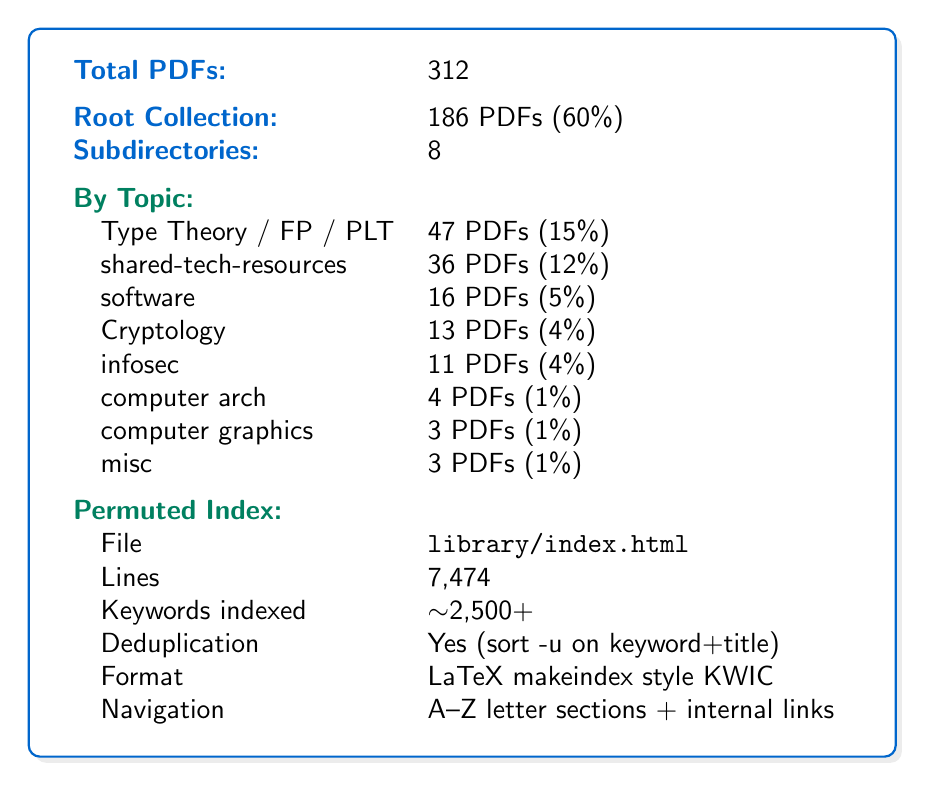
\begin{tikzpicture}
  \node[draw=cyberblue,thick,rounded corners,fill=white,text width=0.85\textwidth,
        inner sep=1em,drop shadow={opacity=0.15}] {
    \begin{tabular}{ll}
      \textbf{\color{cyberblue}Total PDFs:} & 312 \\[0.5em]
      \textbf{\color{cyberblue}Root Collection:} & 186 PDFs (60\%) \\
      \textbf{\color{cyberblue}Subdirectories:} & 8 \\[0.5em]
      \multicolumn{2}{l}{\textbf{\color{cybergreen}By Topic:}} \\
      \quad Type Theory / FP / PLT & 47 PDFs (15\%) \\
      \quad shared-tech-resources & 36 PDFs (12\%) \\
      \quad software & 16 PDFs (5\%) \\
      \quad Cryptology & 13 PDFs (4\%) \\
      \quad infosec & 11 PDFs (4\%) \\
      \quad computer arch & 4 PDFs (1\%) \\
      \quad computer graphics & 3 PDFs (1\%) \\
      \quad misc & 3 PDFs (1\%) \\[0.5em]
      \multicolumn{2}{l}{\textbf{\color{cybergreen}Permuted Index:}} \\
      \quad File & \texttt{library/index.html} \\
      \quad Lines & 7,474 \\
      \quad Keywords indexed & $\sim$2,500+ \\
      \quad Deduplication & Yes (sort -u on keyword+title) \\
      \quad Format & LaTeX makeindex style KWIC \\
      \quad Navigation & A--Z letter sections + internal links \\
    \end{tabular}
  };
\end{tikzpicture}
\end{center}

\section*{Regeneration \& Maintenance}

\begin{description}[leftmargin=2em,style=nextline]
  \item[\textbf{\color{cyberblue}Command:}]
    \texttt{\color{cybergray}\textasciitilde/cyberspace/bin/generate-library-index}

  \item[\textbf{\color{cyberblue}When to Regenerate:}]
    \begin{itemize}[leftmargin=1em]
      \item After adding or removing PDFs from library
      \item When directory structure changes
      \item When updating related documents
    \end{itemize}

  \item[\textbf{\color{cyberblue}Documentation:}]
    Auto-documented in \texttt{\color{cybergray}\textasciitilde/cyberspace/CLAUDE.md}
\end{description}

\section*{Version Control}

\begin{center}
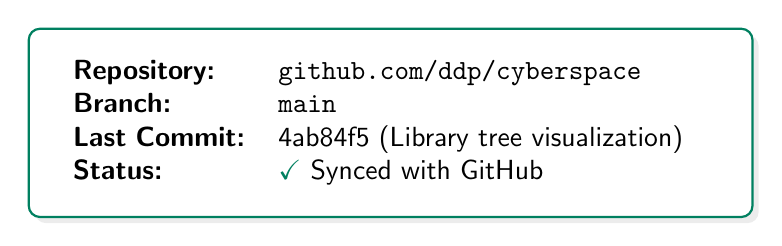
\begin{tikzpicture}
  \node[draw=cybergreen,thick,rounded corners,fill=white,text width=0.7\textwidth,
        inner sep=1em,drop shadow={opacity=0.15}] {
    \begin{tabular}{ll}
      \textbf{Repository:} & \texttt{github.com/ddp/cyberspace} \\
      \textbf{Branch:} & \texttt{main} \\
      \textbf{Last Commit:} & 4ab84f5 (Library tree visualization) \\
      \textbf{Status:} & {\color{cybergreen}\textbf{$\checkmark$}} Synced with GitHub \\
    \end{tabular}
  };
\end{tikzpicture}
\end{center}

\vfill

\begin{center}
{\color{cybergray}\small
Generated \today{} by \textbf{Claude Code Librarian} \\
Part of the \textit{Cyberspace Project} \\
\url{https://github.com/ddp/cyberspace}
}
\end{center}

\end{document}
